\subsection{Styretøj}

De interne signaler for blokken styretøj er beskrevet nedenfor i figur \ref{fig:ibd_styretoej}.

\begin{figure}[h]
\centering
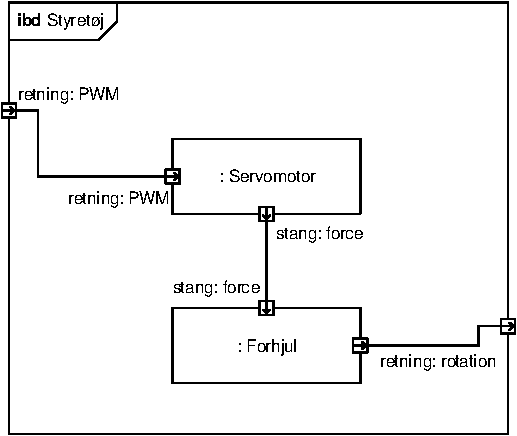
\includegraphics[scale=1]{../fig/diagrammer/bil/ibd_styretoej.pdf}
\caption{IBD for blokken styretøj}
\label{fig:ibd_styretoej}
\end{figure}

\subsubsection{signalbeskrivelse for styretøj}

\begin{table}[h]
	\centering
	\begin{tabularx}{\textwidth}{|l|Z|Z|Z|} \hline
	\textbf{Signal (navn: type)} & \textbf{Funktion} & \textbf{Tolerancer} & \textbf{Kommentarer} \\ \hline
retning: PWM 
	& PWM signal der vha pulsbredden angiver hvilken retning servomotoren skal dreje og dermed hvilken retning bilen skal dreje. 
	& Pulsbredde: 0.5ms – 2.5ms \newline
		Freq = 360Hz \newline
		0.5ms = 18\% Duty cycle (Venstre)\newline
		2.5ms = 90\% Duty cycle (Højre)
	& ~
	\\ \hline
stang: force 
	& Skal overføre kraften fra servomotoren til forhjulene. Dette sker via en stang.
	& -
	& ~
	\\ \hline
retning: rotation
	& Får bilen til at dreje.
	& 30 grader til hhv. venstre og højre $\pm$ 5 grader
	& ~
	\\ \hline
	\end{tabularx}
\end{table}